\message{ !name(written-report.tex)}\documentclass[a4paper]{article}

\usepackage[]{caption}
\usepackage[]{graphicx}
\usepackage[style=apa]{biblatex}
\usepackage[colorlinks=true,citecolor=blue,linkcolor=blue]{hyperref}
\usepackage[]{microtype}
\usepackage[table]{xcolor}
\usepackage[toc,page]{appendix}
\usepackage[capitalise]{cleveref}
\usepackage[margin=1.3in]{geometry}
\usepackage[]{sectsty}
\usepackage[]{setspace}
\usepackage[]{latexsym}
\usepackage[]{ragged2e}

\captionsetup[figure]{
  font = it,
  labelfont = bf
}

\graphicspath{{./graphs/}{./images/}}
\addbibresource{written-report.bib}

\begin{document}

\message{ !name(written-report.tex) !offset(-3) }

\begin{titlepage}
  \Centering{}
  \Large{Raffles Institution \\ Year 5 Project Work \\ Written report} \\
  
\includegraphics[scale=0.5]{ri-school-crest.png} \\
  \huge{The problem of youths falling for online scams, and ways to prevent this.} \\
  \vspace{0.5cm}
  \small{\emph{Word Count: \ldots}} \\
  \vspace{0.5cm} \large{
    \textbf{Authors}: \\
    Alicia Chan \\
    Vera Tay\footnote{Group leader} \\
    Isaac Yeo \\
    Lyu Junwei \\
    Karthik \\
    \vspace{1cm}
    \begin{tabular}{r@{:}l}
      \textbf{Class} & \hspace{1cm} 24S02C \\
    \end{tabular}

  }
\end{titlepage}

\newpage

\pagenumbering{Roman}

\begin{abstract}
  \addcontentsline{toc}{section}{Abstract}
  \noindent
  \ldots?
\end{abstract}

\newpage


\tableofcontents

\newpage

\pagenumbering{arabic}

\section{Identification of problem}
\subsection{Choice of topic}
\paragraph{} Amid the digitalisation of Singapore and the world, there has been
a massive uptick in the number of youths falling for scams in Singapore. This
paper will address the factors contributing to increased scam rates among youths
and potential solutions to stem the problem.

\subsection{Rationale for choice of topic}
\paragraph{} As society becomes increasingly digitalised, many day-to-day
processes are shifting online, from e-commerce \parencite{ITA.2022} to banking
services (Degenhard, 2023). Consequently, young adults are spending more time on
the Internet and falling for online scams. The number of young people falling
for online scams has grown from 15455 total cases in 2021 to a total of 23565 in
2022–more than a 50\% increase \parencite{Tham.2023}. Moreover, it is extremely
difficult for the police to recover the money from scammers: in 2021, more than
90\% of scams originated from overseas, causing the monetary losses to be
largely irreversible \parencite{Begum.2022}. This undermines Digital Defence,
one of the pillars of Singapore’s Total Defence approach \parencite{SCDF.2023},
implying a compromise to Singapore’s security.

\subsection{Significance of problem}
\paragraph{} On the individual level, scam victims tend to feel shame and
helplessness after getting scammed \parencite{CNA.2022}, which puts them at
heightened risk of mental health issues \parencite{SiowDivi.2023}.

\paragraph{} Scam victims also risk thinking that taking advantage of others'
trust is a common occurrence. As a result, victims may start losing trust in
humans, becoming paranoid and keeping to themselves if they normalise scammers'
dishonest behaviour \parencite{SiowDivi.2023}. This may result in a widespread
eradication of once-strong interpersonal relationships.

\paragraph{} To society at large, the substantial amount of money lost to scams
in recent years suggests that youth falling for online scams has a large
economic impact on Singapore; the amount of money lost to online scams has
increased to almost S\$1.3 billion from 2021 to 2022 \parencite{Chua.2023}.

\paragraph{} Youths' current vulnerability to the numerous scam opportunities
results in an overall decrease in the safety of online platforms, with a
possible eradication of trust in online processes. This compromises the
reliability of online services like banking and e-commerce as a whole, which
stops us from taking full advantage of the benefits digitalisation has to offer.
On a global scale, this also endangers Singapore’s reputation as a financial hub
that gives foreigners ``a strong sense of security and comfort''
\parencite{Rikvin}.

\subsection{Rationale for choice of target group}
\paragraph{} As most youth have just entered the workforce, there is
understandably a heightened want and need for money (\cref{fig:incomegraph}),
making scam offers seem attractive. However, this leaves them highly susceptible
to scams: more than 26\% of scam victims are between 20 and 29 years old
\parencite{Chua.2023}, comprising the largest share of 2022 scam victims. They
are especially vulnerable as they ``lack the experience to deal with complex
issues'' \parencite{SiowDivi.2023}, hence they might not be able to cope
emotionally with the consequences of falling for a scam and their mental health
might be especially adversely affected.

\begin{figure}[ht]
  \centering 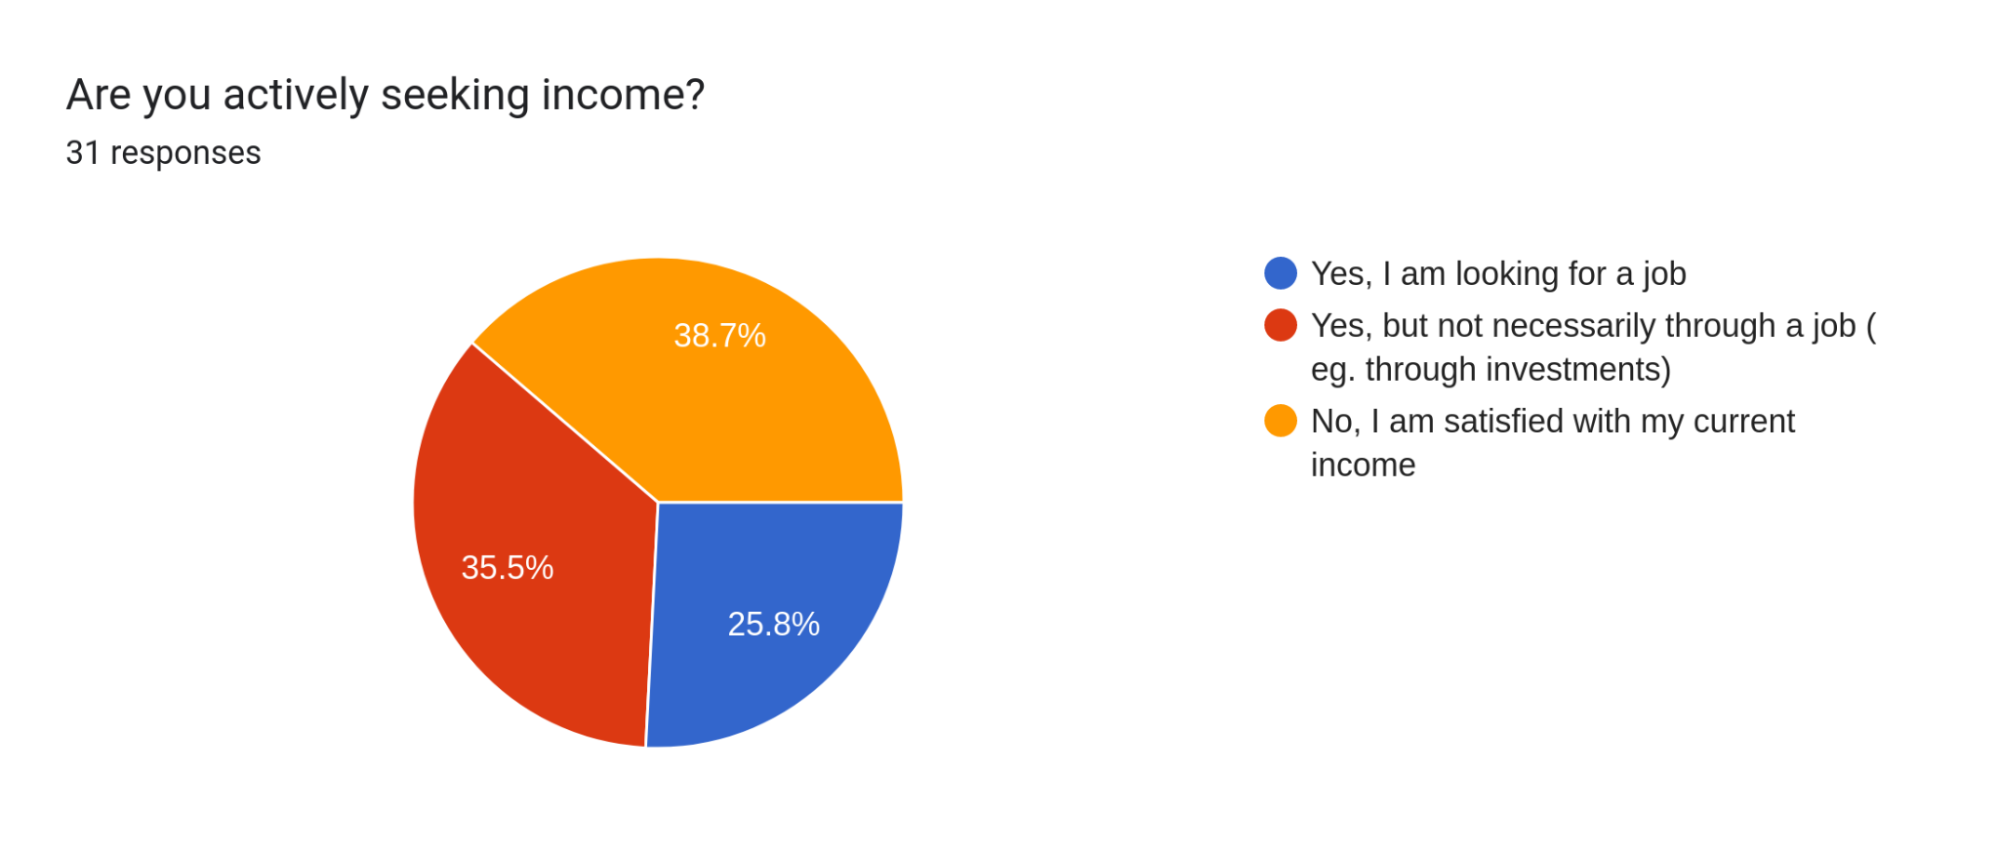
\includegraphics[width=\textwidth]{incomegraph}
  \caption{Chart from survey showing that more than half of the youth we
    surveyed are actively seeking income and hence display a want/need for
    money.}\label{fig:incomegraph}
\end{figure}

\paragraph{} Since youths are just entering the job market and earn relatively
lower salaries, losses from scams may comprise a higher proportion of their
income, resulting in a greater threat to their ability to recover from the
financial blow.

\paragraph{} Considering that this group will shortly be the main contributors
to Singapore’s economy, if the problem is unaddressed, Singapore will suffer
even more unnecessary financial losses in the near future
\parencite{SiowDivi.2023}.

\paragraph{} Lastly, the habits of young adults towards scams may be easier to
reshape than those of older adults due to their higher neuroplasticity
\parencite{GoodTherapy.2019}. Hence, with the wider goal of reducing overall
scam rates in Singapore, it would be most feasible and productive to address
young adults first.

\section{Analysis of target group and the problem}
\subsection{Causual factors}
\subsubsection{Complacent attitudes}
\paragraph{} Young adults tend to have the misconception that they are immune to
scams because they are more tech-savvy compared to older generations, adopting a
“learned carelessness”: “blind spots caused by being digitally savvy”
\parencite{Yuan.2023}. Consequently, their complacency is perpetuated by the
stereotype that the elderly are the most common victims of scams. Young adults’
“curiosity” and “propensity for risk-taking” cause them to “hold the belief that
scams will not affect them personally, which renders them more vulnerable”
\parencite{Cheung.2023}. Since they are less careful online
\parencite{Carlson.2022}, they easily fall for scams.

\paragraph{} Our survey results corroborate youths’ self-perceived competency
towards scams (\cref{fig:scamknowledgegraph}). Due to their complacency, young
adults are also less willing to learn more about identifying and preventing
scams.

\begin{figure}[ht]
  \centering 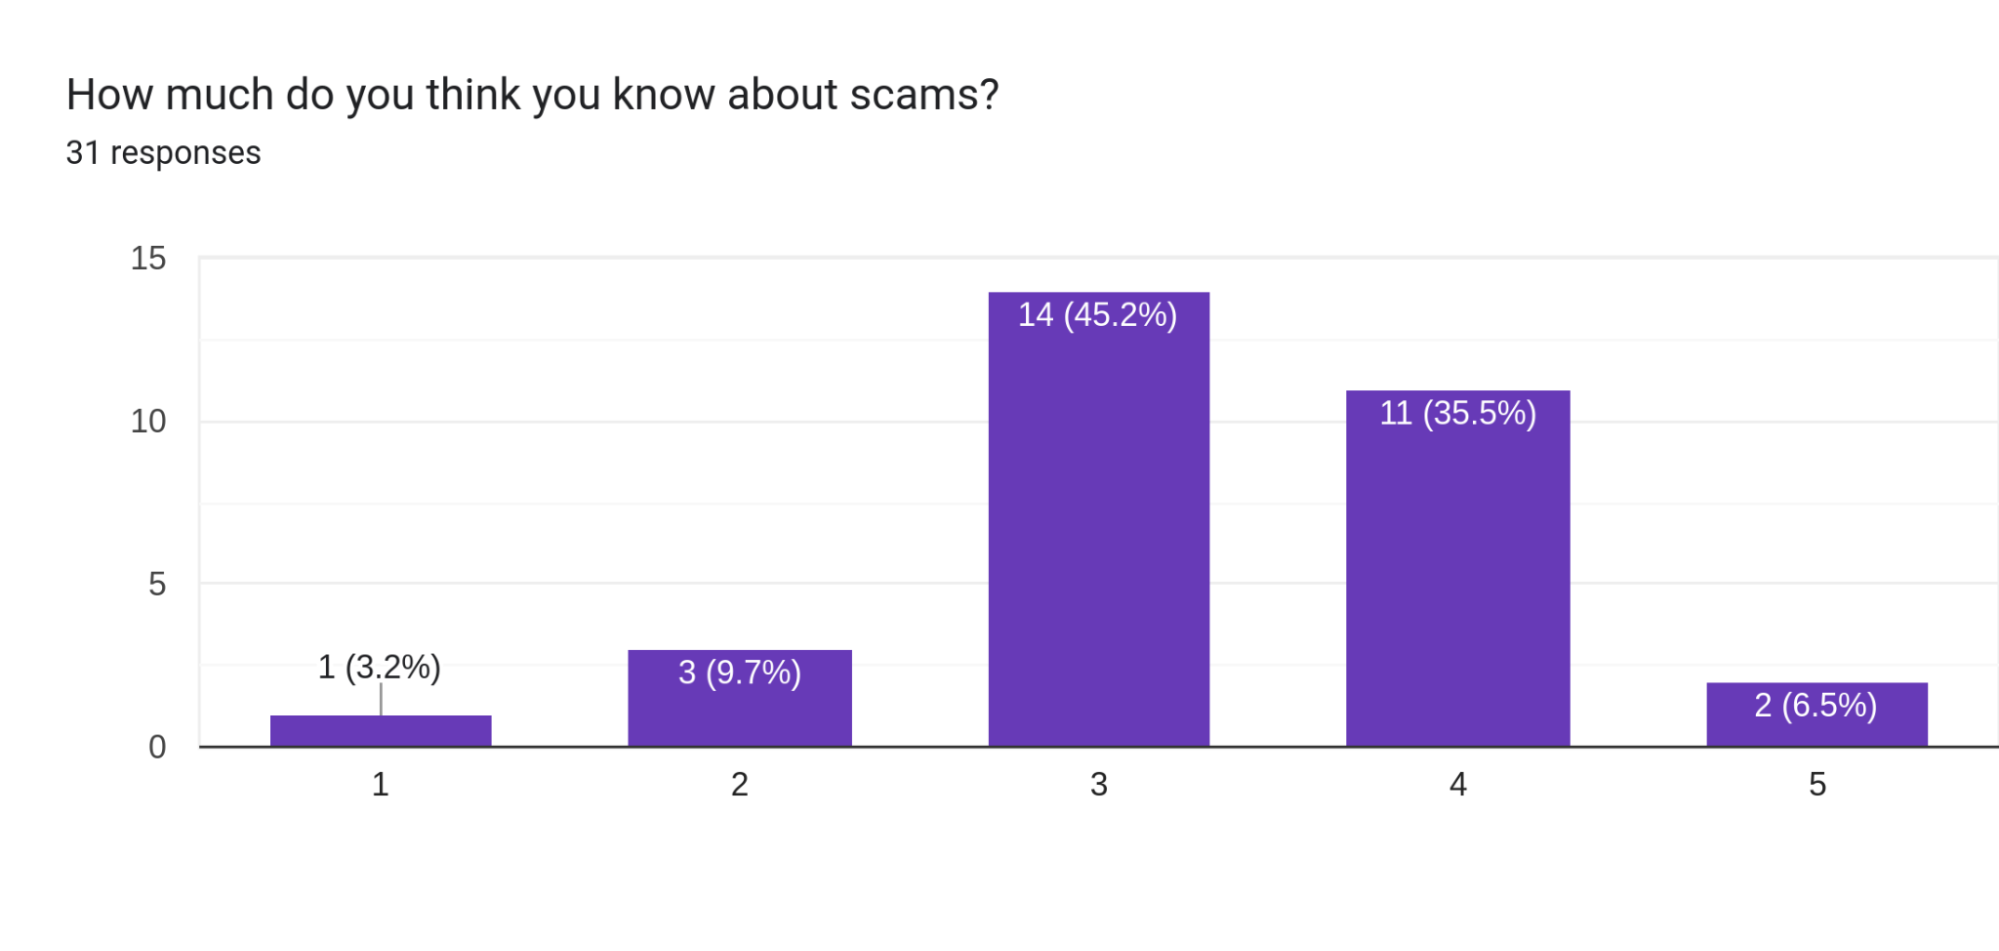
\includegraphics[width=\textwidth]{scamknowledgegraph}
  \caption{Bar chart showing majority of respondents indicating they have at
    least adequate knowledge towards scams, where 1 means ``severely
    insufficient knowledge'' and 5 means ``highly comprehensive knowledge''.
    This shows youths' complacency in their ability to identify scams; most
    think they have the minimal skills required to avoid falling prey to scams,
    but scam rates among youths suggest
    otherwise.}\label{fig:scamknowledgegraph}
\end{figure}


\subsubsection{Lack of technical knowledge}
\paragraph{} Youths are unable to recognise how common scams such as job and
investment scams work. For instance, despite initial payouts to victims (which
``[lures] them into providing more funds'') being a common scam strategy, youths
still fall for this ploy, as evidenced by job and investment scams being among
the top scams in 2022 \parencite{Hui.2023}.

\paragraph{} Additionally, scammers constantly devise new tactics, such as the
``fake friend call scam'' which has become overwhelmingly popular
\parencite{Goddard.2023}. Thus, without proactive knowledge-seeking from youth,
information on scam prevention quickly becomes irrelevant. Therefore, youth lack
the knowledge to prevent scams both in the short and long term.

\subsection{Current measures and gaps}
\subsubsection{NCPC's campaign}
\paragraph{} The National Crime Prevention Council (NCPC) has launched an
anti-scam campaign with the 2023 tagline ``I can ACT against scams''
\parencite{Sun.2023} as well as a website called ScamAlert \parencite{NCPC}.

\paragraph{} However, the campaign is intended for the general public and is
consequently not tailored for young adults, as suggested by the diversity of the
ambassadors of the campaign (\cref{fig:scamalert}). The underlying complacency
in young adults is not addressed, as the idea that anyone can be a target of
scams is not a focal point.

\paragraph{} Additionally, certain sections of the ScamAlert website can be
wordy, possibly resulting in low engagement with youths who tend to have a
shorter attention span \parencite{ChowHari.2022} and may be unwilling to read
through the long paragraphs.

\begin{figure}[ht]
  \minipage[t]{0.45\textwidth}
  \centering 
\includegraphics[width=\textwidth]{scamalert}
  \caption{Main page of the ``ACT NOW'' section on the ScamAlert website with
    representatives of varying ages, showing that it is not specifically
    targeted to our target group.}\label{fig:scamalert}
  \endminipage\hfill
  \minipage[t]{0.45\textwidth}
  \centering 
\includegraphics[width=\textwidth]{scamalertwordy}
  \caption{Example of a wordy information page on the ScamAlert website that
    youths would be unwilling to read.}\label{fig:scamalertwordy}
  \endminipage{}
\end{figure}

\subsubsection{The Straits Times' ``STOP SCAMS'' initiative}
\paragraph{} ST\footnote{The Straits Times}'s ``STOP SCAMS'' initiative features
stories of people getting scammed and advises readers on how to avoid such
scams. At the end of each article, the ScamAlert website is mentioned as a
resource.

\begin{figure}[ht!]
  \minipage[b]{0.45\textwidth} \centering
  
\includegraphics[width=\textwidth]{stopscams1} \endminipage\hfill
  \minipage[b]{0.45\textwidth} \centering
  
\includegraphics[width=\textwidth]{stopscams2} \endminipage{}
  \caption{Examples of “Stop Scams” features in the print version of ST, which
    is not commonly accessed by young adults ages 20-29}\label{fig:stopcams}
\end{figure}

\paragraph{} While this initiative is also helpful and informative, its reach
may be limited. Only 16\% of Generation Z and 24\% of millennial readers access
ST physically \parencite{Ho.2021}. As it is inherently not guaranteed that these
scam articles reach online readers, the engagement with ST’s initiative may be
low.

\paragraph{} Put simply, NCPC and ST's initiatives do not consider youths'
habits, learning styles and preferences, resulting in low visibility of these
resources to youths.

\subsection{Our approach}
\paragraph{} We have a two-pronged approach:

\subsubsection{Changing attitudes}
\paragraph{} To incite behavioural change such that youth would act more
cautiously when facing scams, a mindset change is crucial
\parencite{ConnorBernal.2020}. Thus, we first need to change youths’ complacent
attitudes towards scams and ensure that they are aware that they are vulnerable
to scams.

\subsubsection{Educate}
\paragraph{} When youths are aware of the need to learn more about scams,
\emph{Educate} plugs any knowledge gaps that youths may have with regards to
identifying and avoiding scams. Even sophisticated scams have telltale
indicators which can be taught to youths, such as ``soliciting offers, asking
[for] personal information, [and the] use of hyperlinks''
\parencite{DatarColeRogers.2014}, showing that educating willing youths can
increase their ability to identify and avoid scams.

\newpage
\subsection{Flowchart}
\begin{figure}[ht!]
  \centering 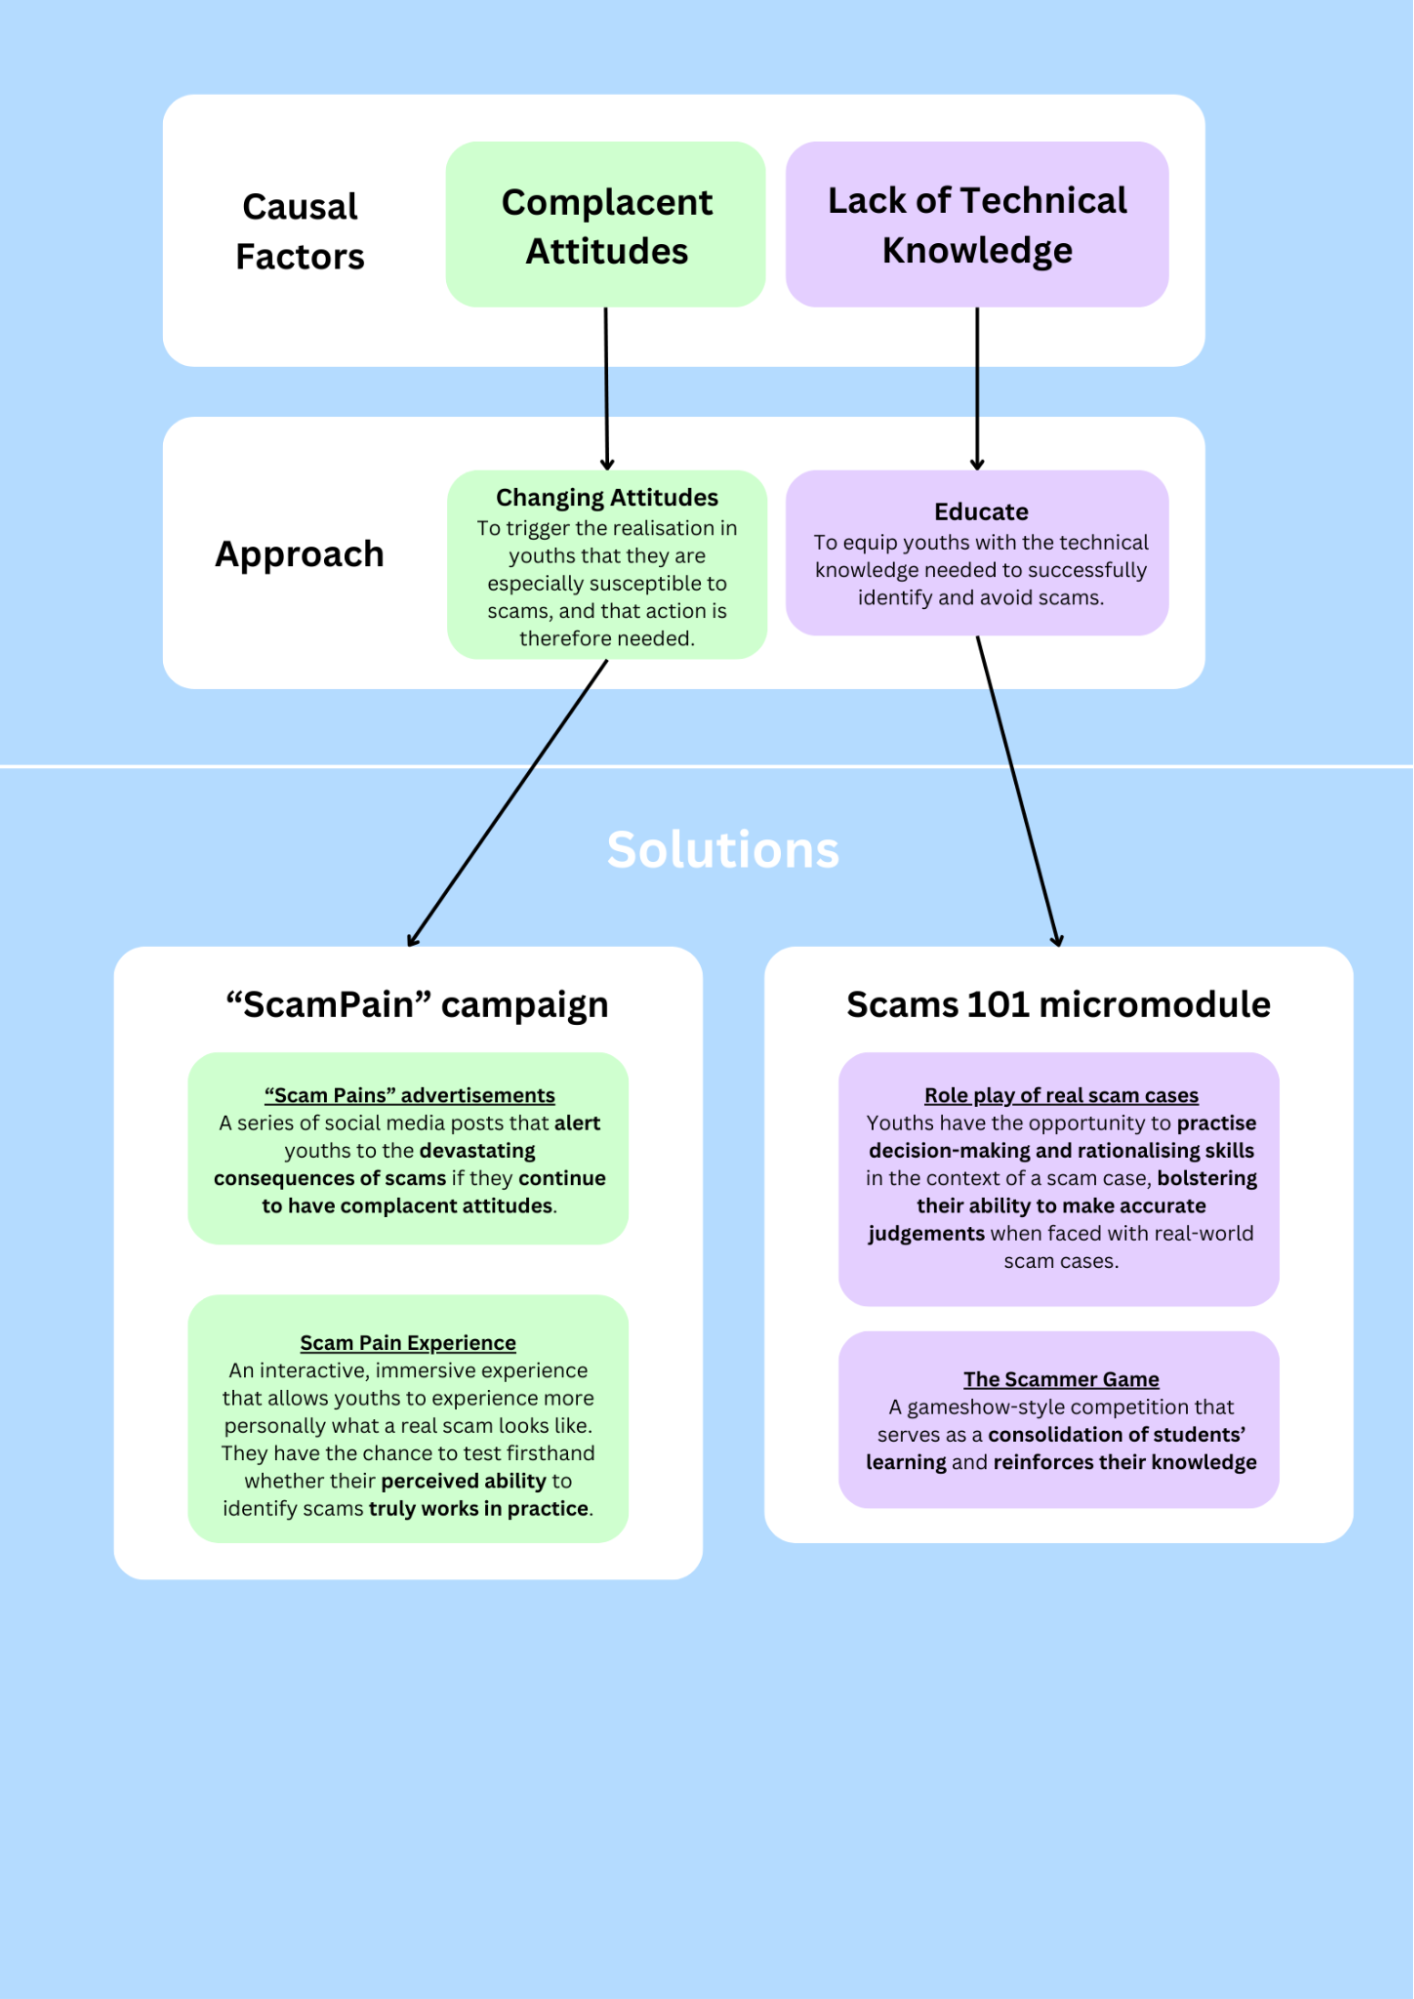
\includegraphics[width=\textwidth]{flowchart}\label{fig:flowchart}
\end{figure}

\section{Changing attitudes: ``ScamPain'' campaign}
\subsection{Objectives}
\subsection{Details}
\subsubsection{Advertisments}
\subsubsection{Immersive experience}
\subsection{Evaluation}

\section{Educate: Scams 101 micromodule}
\subsection{Objectives}
\subsection{Rationale}
\subsection{Details}
\subsection{Evaluation}

\section{Conclusion}
\subsection{Overall evaluation}
\subsection{Future development}

\newpage

\nocite{*} \printbibliography[heading=bibintoc,title={References}]

\newpage

% TC:ignore

\begin{appendices}
\end{appendices}


% TC:endignore
\end{document}

\message{ !name(written-report.tex) !offset(-305) }
